\chapter{基于预训练辅助模型的Token表征学习}
\label{chap:Token}
本章主要对本文提出的基于预训练辅助模型的Token表征学习方法进行详细介绍,首先介绍其研究动机,接着阐述其方法设计,以及具体的实现过程,最后介绍实验验证过程和结果。

\section{研究动机}
\label{sec:Motivation}

基于Token的代码表征方法本质上就是将源代码转换为一系列词法单元Token组成的序列,并对Token序列进行代码分析。类似于自然语言技术处理文本,由于源代码中存在大量用户自己定义的标识符,不同用户的命名习惯不同,在对源代码的词法单元建模时,会产生一个规模巨大且稀疏的词汇表。该词汇表的规模会直接影响代码分析任务的效率,因此现有方法大多都对Token进行规范化,比如将变量名用统一的标识符来代替,从而降低词汇表的规模。但是后续神经网络模型训练过程中,当出现某个词汇在词汇表中没有出现过,那么神经网络模型就无法对齐建模,即出现了在词汇表中不存在的Token,集外词(Out-of-vocabulary,简称OOV)问题。有研究\cite{RJXB202205011}发现,针对代码表征中的集外词问题,在经典BigcloneBench\cite{7332459}数据集中OOV比率高达62.68\%,在OJClone数据集\cite{WOS:000485474201046}中OOV比率达到了16.82\%。

为了解决OOV问题,本文打算使用预训练模型增加词汇表的大小。近期,研究人员在大规模语料库上预训练各种语言模型,在解决各种自然语言处理任务方面取得了良好进展\cite{zhao2023survey}。在表征学习领域,也有基于大规模预训练模型提升代码表征能力的方法被提出。InferCode\cite{9402028}将自然语言处理中的自监督学习思想引入到代码的抽象语法树的表示中, 通过预测从AST上下文中自动识别的子树来训练代码表征,并且使用AST的子树作为训练标签,从而无需任何人工标记工作。该预训练InferCode模型可以应用于下游的无监督学习,例如代码聚类、代码克隆检测、跨语言代码搜索等。GraphCodeBERT\cite{guo2021graphcodebert}方法提出了一个基于数据流的代码表征预训练模型,与抽象语法树不同,数据流包含代码变量间“值从哪里来”的语义特征,并不会带来深层次不必要的复杂信息,使用该特征可以更有效的生成代码表征。然而这些预训练模型通常存在参数规模庞大, 训练及使用代价大的问题。

因此,针对集外词OOV问题,本文提出了一种轻量级的基于预训练辅助模型的Token表征学习方法,该方法在提升代码表征能力的同时,并不会引入过多参数,造成模型训练代价高的问题。

\section{Token表征方法设计}
\label{sec:Token}
本节将主要介绍基于预训练辅助模型的Token表征学习方法的详细设计,首先介绍该方法的整体框架,并分别从预训练辅助词嵌入、Token代码表征两方面介绍具体设计。

\subsection{框架概述}
\label{subsec:TokenOverview}
本文提出的基于预训练辅助模型的Token表征学习方法的整体框架如图\ref{fig:tokenframework}所示。该框架的输入是代码片段对应的Token序列,输出是对应的属性特征向量,主要包括预训练辅助词嵌入、Token代码表征两个阶段。

\begin{figure}[H]
  \centering
  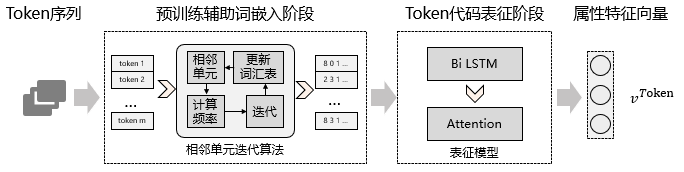
\includegraphics[width=0.95\textwidth]{figures/tokenframework}
  \caption{基于预训练辅助模型的Token表征学习框架}\label{fig:tokenframework}
\end{figure}

首先,预训练辅助词嵌入阶段以代码片段的Token序列作为训练数据,构建一个预训练辅助词嵌入模型。该模型的输入是代码片段对应的Token序列,输出为与输入对应的Token词嵌入向量。然后通过对模型的训练,使得该模型具有正确识别Token的能力,并将该模型保存下来。需要注意的是,为了减少集外词OOV问题,本文对模型采用相邻单元迭代算法,即,通过多次迭代来更新词汇表。

其次,Token代码表征阶段以Token词嵌入向量作为训练数据,构建一个Token表征模型。该模型的输入是Token序列对应的词向量,输出为一个固定长度的密集向量用来表示代码的属性特征。需要注意的是,本文选用的AttBiLSTM神经网络,主要包含两个部分:双向长短时记忆部分(BiLSTM)和自注意力机制部分(Attention),前者主要目的是同时捕获序列的双向语义信息,后者的主要目的是总结序列的输入特征,并将每个代码片段缩减为一个单一的密集向量。

在上述框架中,本文的创新点主要体现在预训练辅助词嵌入阶段的相邻单元迭代算法、Token代码表征阶段的模型设计两方面,下面将围绕这两个创新点来阐述本文的方法。

\subsection{预训练辅助词嵌入设计}
\label{subsec:Model}

相邻单元迭代算法是预训练辅助词嵌入阶段的重点,也是减少集外词OOV问题的关键。下面对相邻单元迭代算法进行介绍。

在模型训练之前,通过选取合适的模型从代码语料库中学习基本单元的语法语义信息,以及这些单元之间的联系,最终给出一份单词-向量形式的词汇表,从而减少出现集外词问题的概率。

具体的,第一次迭代选择相邻的两个token组合为一个单元,查找出最频繁的token组合确定为一个组合单元,并将组合单元更新到词汇表中,然后二次迭代,每次迭代在原来的基本单元上再组合一个新的邻近token作为新的判断单元,每次迭代都会更新词汇表。在得到词汇表之后,根据词汇表获取每个单元的向量表示。


\begin{algorithm} 
	\caption{Iterative Method of adjacent tokens} 
	\label{alg1} 
	\begin{algorithmic}
		\REQUIRE Tokens sequence $T$,the number of iterations $n$ 
		\ENSURE $y = x^n$ 
		1:\STATE $y \gets 1$ 
		\IF{$n < 0$} 
		\STATE $X \gets 1 / x$ 
		\STATE $N \gets -n$ 
		\ELSE 
		\STATE $X \gets x$ 
		\STATE $N \gets n$ 
		\ENDIF 
		\WHILE{$N \neq 0$} 
		\IF{$N$ is even} 
		\STATE $X \gets X \times X$ 
		\STATE $N \gets N / 2$ 
		\ELSE[$N$ is odd] \STATE $y \gets y \times X$ 
		\STATE $N \gets N - 1$ 
		\ENDIF 
		\ENDWHILE 
	\end{algorithmic} 
\end{algorithm}

\subsection{Token代码表征设计}
\label{subsec:Token}

将token序列对应的向量输入到Bi LSTM网络中,经过Bi LSTM学习哪些信息应该被记住哪些信息应该被遗忘,最终得到每个基本单元包含语义信息和上下文信息的向量表示。Bi LSTM由一个正向的LSTM和一个反向的LSTM组成,主要思想是通过把序列向前、向后分别输入给两个独立的递归网络,这两个子网络连接到一个输出层,在每个词的输出部分把两个子网络的输出信息进行整合,这样网络就同时拥有了序列中每个词的过去时刻信息和未来时刻信息。Bi LSTM可以捕获到序列前后的关系依赖,将代码片段的Token序列转换为可相互比较的向量。

\section{Token表征方法具体实现}
\label{sec:achieve}
本文提出的基于预训练辅助模型的Token表征学习方法的实现如图\ref{fig:token}所示。该方法的输入是代码片段$C_{a},C_{b}$对应的Token序列,输出是$C_{a},C_{b}$对应的属性特征向量,整体采用Siamese架构,两个子网络共享权值。该框架主要包括预训练辅助词嵌入、Token代码表征两个阶段。

\begin{figure}[H]
  \centering
  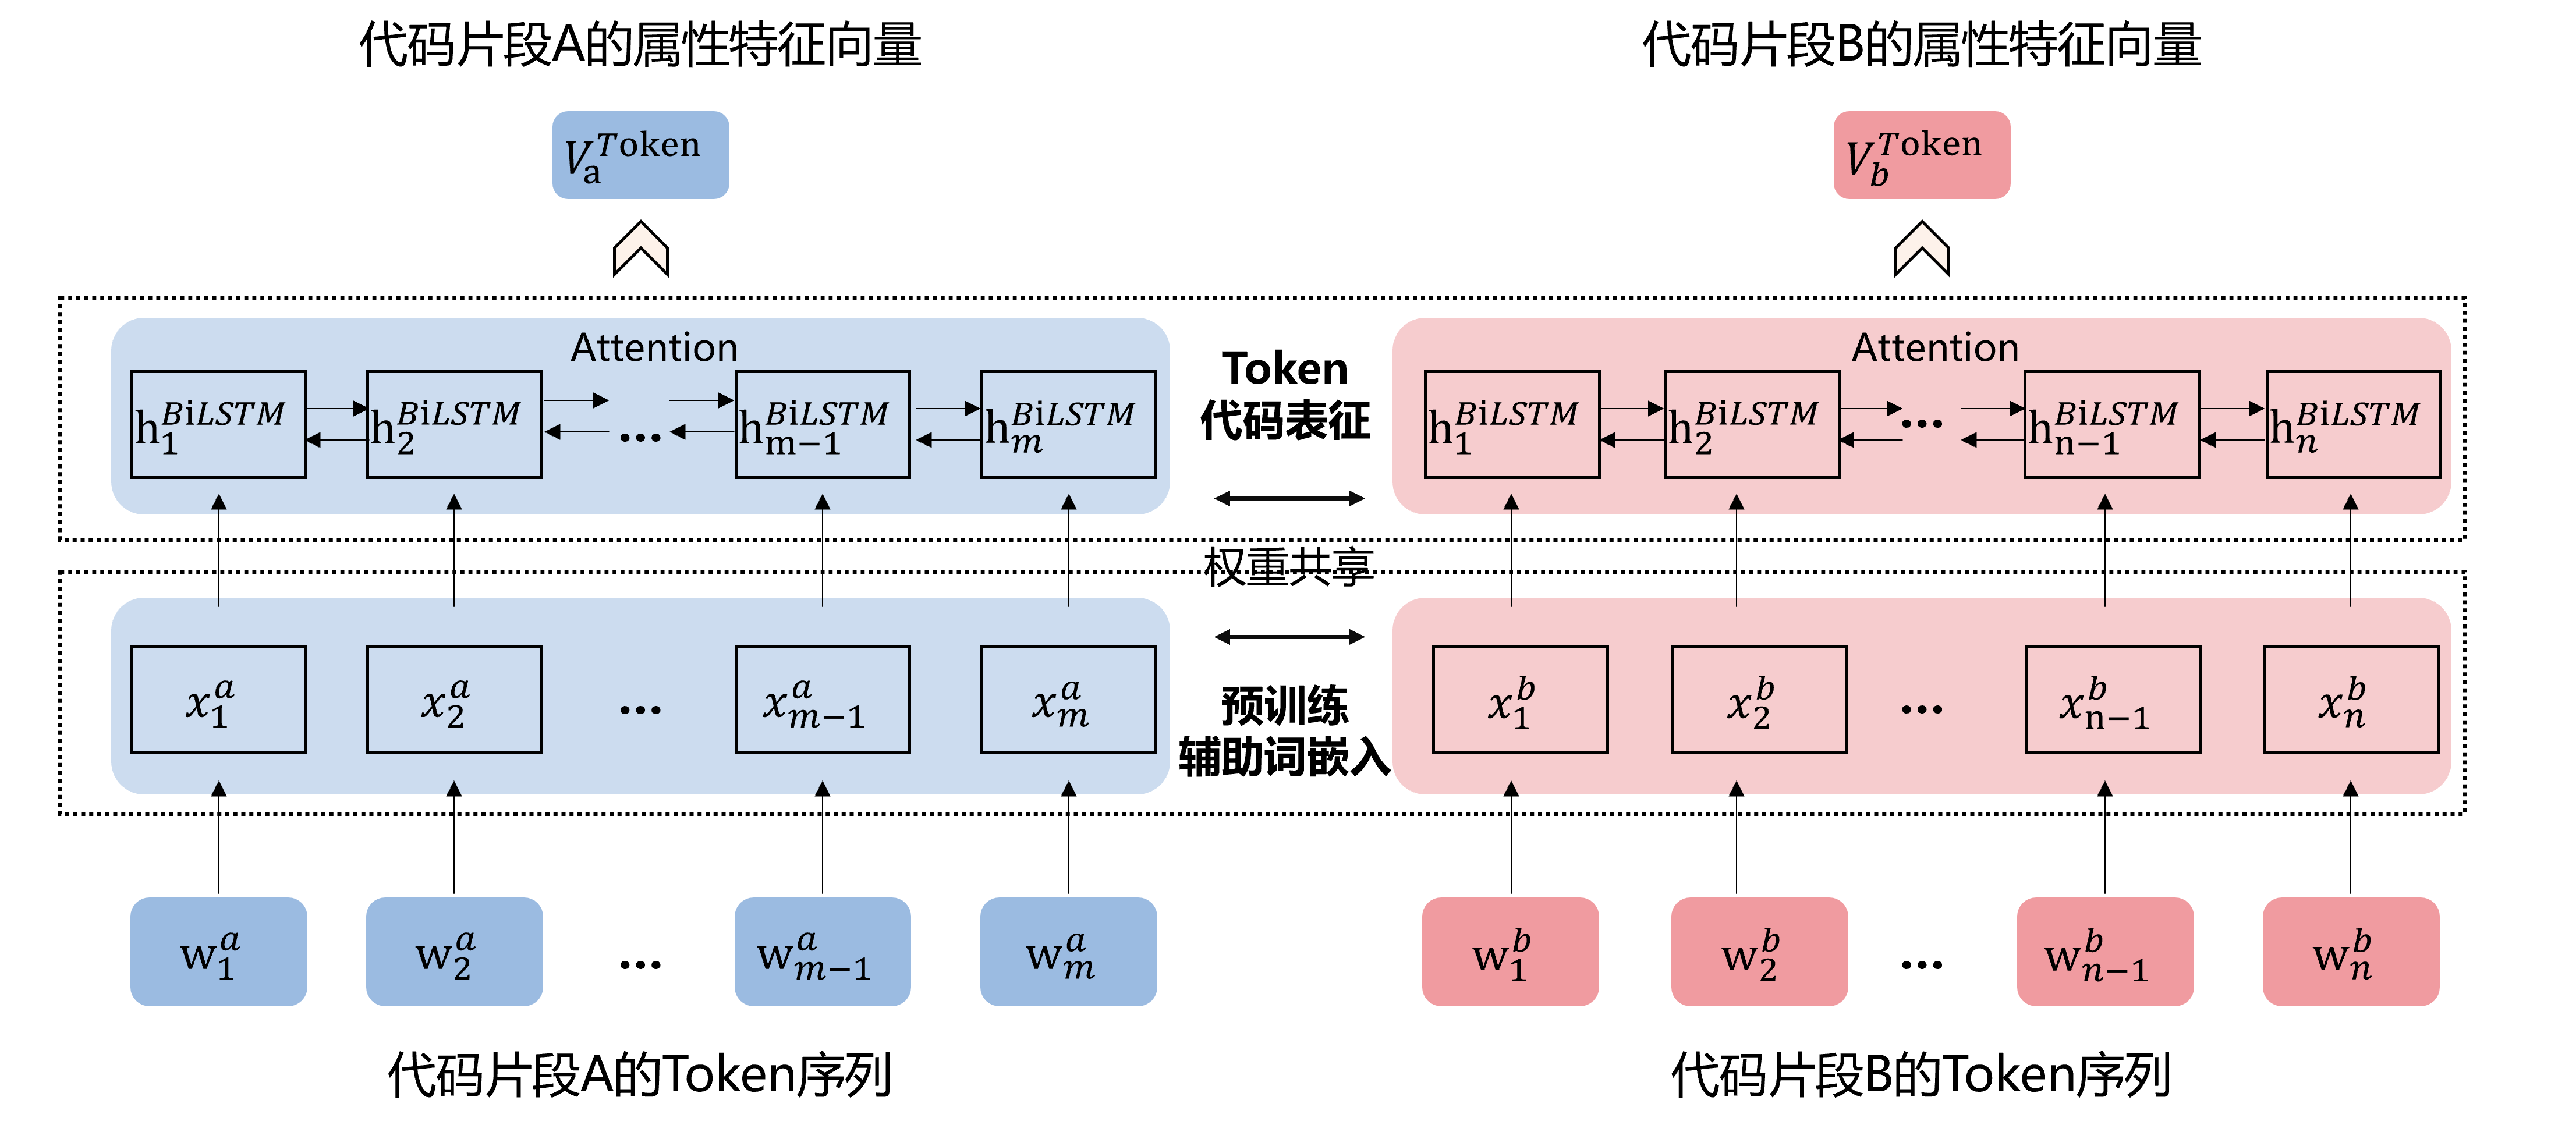
\includegraphics[width=0.95\textwidth]{figures/token}
  \caption{基于预训练辅助模型的Token表征学习方法实现}\label{fig:token}
\end{figure}


\section{实验验证}
\label{sec:Experiment}
为了验证基于预训练辅助模型的Token表征方法的有效性,本节展开实验验证。首先,介绍了实验整体的环境配置、数据集,以及实验评估;接着,对基于预训练模型的Token表征方法进行了消融实验。

\subsection{实验环境}
\label{subsec:Environment}
本章的实验验证均运行于Linux系统下,其系统硬件配置如表\ref{tab:environment}所示。

\begin{table}[H]
  \centering
  \caption{实验环境配置} 
  \label{tab:environment}
  \begin{tabular*}{0.6\textwidth}{@{\extracolsep{\fill}}cc}
  \toprule
    环境			&配置		\\
  \midrule
    操作系统		&Ubuntu 20.04 \\
    处理器			&Intel Core i9-12900KF × 24 \\
    内存			  &31.1G \\
    显卡			  &NVIDIA  \\
    磁盘			  &1TB \\
  \bottomrule
  \end{tabular*}
\end{table}

\subsection{实验数据集}
\label{subsec:Dataset}
为了验证预训练辅助模型在Token层面上表征学习的有效性,本文面向代码克隆检测任务对预训练辅助模型进行分析和评估,选取的实验数据为POJ104数据集。如表\ref{tab:dataset}所示,POJ104数据集是一个基于C语言所构建的大型数据集。OJ系统是一个以编程教学为目的公开评判系统,共存在104个编程问题,针对每个编程问题,学生们通过在线提交自己的代码来尝试解决,同时OJ系统将自动判断提交源代码的正确性和有效性。对于OJ系统中同一个编程问题来说,其所有正确提交的代码都为克隆代码,对于不同的编程问题所提交的代码,即为非克隆代码。POJ104数据集针对每一个编程问题,均提供500个学生提交源代码,即共有52000个样本。

\begin{table}[H]
  \centering
  \caption{POJ104数据集} 
  \label{tab:dataset}
  \begin{tabular*}{0.6\textwidth}{@{\extracolsep{\fill}}cc}
  \toprule
    代码			&属性		\\
  \midrule
    Dataset			&POJ104数据集 \\
    Language    &C \\
    Program			&52000 \\
    Classes			&104 \\
    Max tokens			&8737 \\
    Avg tokens			&245 \\
  \bottomrule
  \end{tabular*}
\end{table}

得到POJ104数据集后,本文首先对数据集进行初步筛选,去掉其中包含乱码的样本,共得到51485个源代码样本。然后对源代码进行预处理,删除样本中包含的空白行和注释等多余代码,并将数据集保存到一个program.pkl文件中,program.pkl文件中一共包含51485行×3列的数据集,每一行数据代表一个源代码样本,第一列为源代码id,第二列保存源代码样本code,第三列为源代码的标签label,即属于哪一个编程问题。接着,本文随机两两组合同一标签label的源代码,组成5200个真克隆对,随机组合不同标签的源代码组成44800个假克隆对,一共给包含50000个克隆对,并将其保存到oj\_clone\_ids.pkl文件中,oj\_clone\_ids.pkl文件中一共包含50000行×3列的数据集,每一行数据代表一个克隆对样本,第一列为源代码id1,第二列为源代码id2,第三列为克隆对的标签label,真克隆对标签为1,假克隆对标签为0。最后,依据随机种子将数据集按照3:1:1划分为训练集、测试集、验证集,其中的正负样本数如下表\ref{tab:ClonePairs}所示。

\begin{table}[H]
  \centering
  \caption{本文预处理后的POJ104数据集正负样本数} 
  \label{tab:ClonePairs}
  \begin{tabular*}{0.8\textwidth}{@{\extracolsep{\fill}}cccc}
  \toprule
    数据集			&真克隆对		&假克隆对		&克隆对数 \\
  \midrule
    训练集train			&3162	  &26838		&30000 \\
    测试集test			&1022		&8978		  &10000 \\
    验证集dev			  &1016		&8984		  &10000 \\
    总计            &5200	  &44800	  &50000 \\
  \bottomrule
  \end{tabular*}
\end{table}

\subsection{评估指标}
\label{subsec:Index}
代码克隆检测问题是二分类问题,因此本文采用准确率(Accuracy)、精确率(Precision)、召回率(Recall)、F1值四个评估指标来度量实验结果,其中使用了混淆矩阵中的TP、FN、FP、TN,如表\ref{tab:ConfusionMatrix}所示。

\begin{table}[H]
  \centering
  \caption{分类问题的混淆矩阵} 
  \label{tab:ConfusionMatrix}
  \begin{tabular*}{0.7\textwidth}{@{\extracolsep{\fill}}ccc}
  \toprule
  \multirow{2}{*}{实际值} & \multicolumn{2}{c}{预测值} \\
  \multirow{2}{*}{} & 正样本(P) & 负样本(N) \\
  \midrule
    正样本(P)			&TP	  &FN		 \\
    负样本(N)			&FP		&TN		 \\
  \bottomrule
  \end{tabular*}
\end{table}

其中,混淆矩阵中的真阳性、假阳性、真阴性、假阴性代表的含义如下:

真阳性(True Positive, TP):样本实际为正样本,并且被模型预测为正样本,即实际上标记为真克隆对并且被检测出来为真克隆对的代码对。
 
假阳性(False Positive, FP):样本实际为负样本,但是被模型预测为正样本,即实际上标记为假克隆对但是被检测出来为真克隆对的代码对。
 
假阴性(False Negative, FN):样本实际为正样本,但是被模型预测为负样本,即实际上标记为真克隆对但是被检测出来为假克隆对的代码对。
 
真阴性(True Negative, TN):样本实际为负样本,并且被模型预测为负样本,即实际上标记为假克隆对并且被检测出来为假克隆对的代码对。

准确率(Accuracy)表示预测为正的样本中真实值为正的比率,计算公式如\ref{e5}所示:
\begin{equation}\label{e5}
  Accuracy = \frac{TP+TN}{TP+FN+FP+TN} 
\end{equation}

精确率(Precision)表示正确检测到的代码克隆数量占全部预测为代码克隆的比例,计算公式如\ref{e6}所示:
\begin{equation}\label{e6}
  Precision = \frac{TP}{TP+FP} 
\end{equation}

召回率(Recall)表示正确检测到的代码克隆数量占总体实际代码克隆数量的比例,计算公式如\ref{e7}所示:
\begin{equation}\label{e7}
  Recall = \frac{TP}{TP+FN} 
\end{equation}

精确率(Precision)和召回率(Recall)指标有时候会出现的矛盾的情况,这样就需要综合考虑两者的表现,最常见的方法就是F1,精确率和召回率的加权调和平均,用于评价分类模型的好坏。计算公式如\ref{e8}。
\begin{equation}\label{e8}
  F1 = \frac{2*Precision*Recall}{Precision+Recall} 
\end{equation}

\subsection{预训练辅助模型消融实验结果}
消融对比实验:体现改进的辅助模型的有效性,如图\ref{tab:category}
基于Token的Bi LSTM
基于Token的+预训练辅助模型的Bi LSTM

\begin{table}[H]
  \centering
  \caption{预训练辅助模型实验结果} 
  \label{tab:category}
  \begin{tabular*}{0.8\textwidth}{@{\extracolsep{\fill}}cccc}
  \toprule
    对比			&P		&R		&F1 \\
  \midrule
    基于Token的Bi LSTM			&0.xx	&0.xx		&0.xx \\
    基于Token的+预训练辅助模型的Bi LSTM			&0.xx		&0.xx		&0.xx \\
  \bottomrule
  \end{tabular*}
\end{table}

\section{本章小结}
\label{sec:Summary3}
本章主要对RLCCD中基于预训练辅助模型的Token表征学习方法的设计与实现进行详细阐述。首先介绍了Token维度的研究动机,其次介绍了Token表征学习的方法设计,具体论述了其整体框架、预训练辅助模型、表征学习,接着开展实验验证,结果表明了此方法的有效性和模型的准确性。
